\chapter{\texorpdfstring{Invariants}{Invariants}}
\label{ch:14}
\lecturemeta{Lezione 14 \quad\textbullet\quad 2026-07-03 \quad\textbullet\quad Roberto Bruni}{Petri nets · Esparza, \emph{Free Choice Petri Nets} (optional)}

Con l'algebra delle matrici (\hyperref[ch:11]{11 — Net Matrices}) abbiamo visto che si può ragionare sulle reti \textbf{senza} costruire l'occurrence graph. Questa lezione porta l'idea al suo culmine con gli \textbf{invarianti}: certe quantità che \textbf{restano costanti} durante ogni esecuzione, calcolabili direttamente dalla struttura della rete. Un solo invariante può dimostrare in una riga proprietà che altrimenti richiederebbero di esplorare tutti gli stati — per esempio "questa rete è bounded" o "questa marcatura non è raggiungibile". Studieremo due tipi duali: gli \textbf{S-invariant} (sui place) e i \textbf{T-invariant} (sulle transizioni).

\begin{boxdefinition}{Invariante}
Un \textbf{invariante} di un sistema dinamico è un'asserzione che \textbf{vale in ogni stato raggiungibile}. Esempi fuori dai Petri net: il perimetro e il numero di lati di un poligono restano invarianti se lo ruoti o lo trasli (ma il perimetro \emph{cambia} se lo scali). In un Petri net, gli stati sono le marcature e le "mosse" sono gli scatti: un invariante è una proprietà vera per \emph{tutte} le marcature raggiungibili.
\end{boxdefinition}

\begin{boxnote}{Anche le proprietà comportamentali sono invarianti}
Liveness, deadlock-freedom, boundedness e ciclicità sono tutte \textbf{ereditarie}: se valgono da $M_0$, valgono anche ripartendo da \emph{qualsiasi} marcatura raggiungibile $M$. (Es. se il sistema è live e $M \in [M_0\rangle$, allora anche $(P,T,F,M)$ è live: ogni $M'$ raggiungibile da $M$ è raggiungibile da $M_0$, dove la liveness vale.) La \textbf{ciclicità} — $\forall M \in [M_0\rangle.\; M_0 \in [M\rangle$, cioè "si può sempre tornare a $M_0$" — è un altro esempio di questa famiglia.
\end{boxnote}

Ma l'interesse vero sono gli \textbf{invarianti strutturali}, calcolati dalla sola struttura della rete (l'incidence matrix) e \textbf{indipendenti dalla marcatura iniziale}.

\begin{boxtip}{Perché gli invarianti}
\begin{itemize}
\item Si calcolano \textbf{efficientemente} (tempo polinomiale per una base), a differenza della raggiungibilità (EXPSPACE-hard).
\item Sono \textbf{indipendenti dalla marcatura iniziale}: una proprietà strutturale con conseguenze comportamentali.
\item Ragione didattica (dice il prof): \emph{capisci davvero un modello solo quando lo pensi in termini di invarianti.}
\end{itemize}
\end{boxtip}

\section{\texorpdfstring{S-invariant: pesi sui place, somma conservata}{S-invariant: pesi sui place, somma conservata}}

L'idea di un \textbf{S-invariant} (o \emph{place-invariant}) è assegnare un \textbf{peso} a ogni place in modo che la \textbf{somma pesata dei token} non cambi mai, qualunque scatto avvenga. L'immagine mentale migliore è quella delle \textbf{monete}.

\begin{figure}[!htb]
\centering
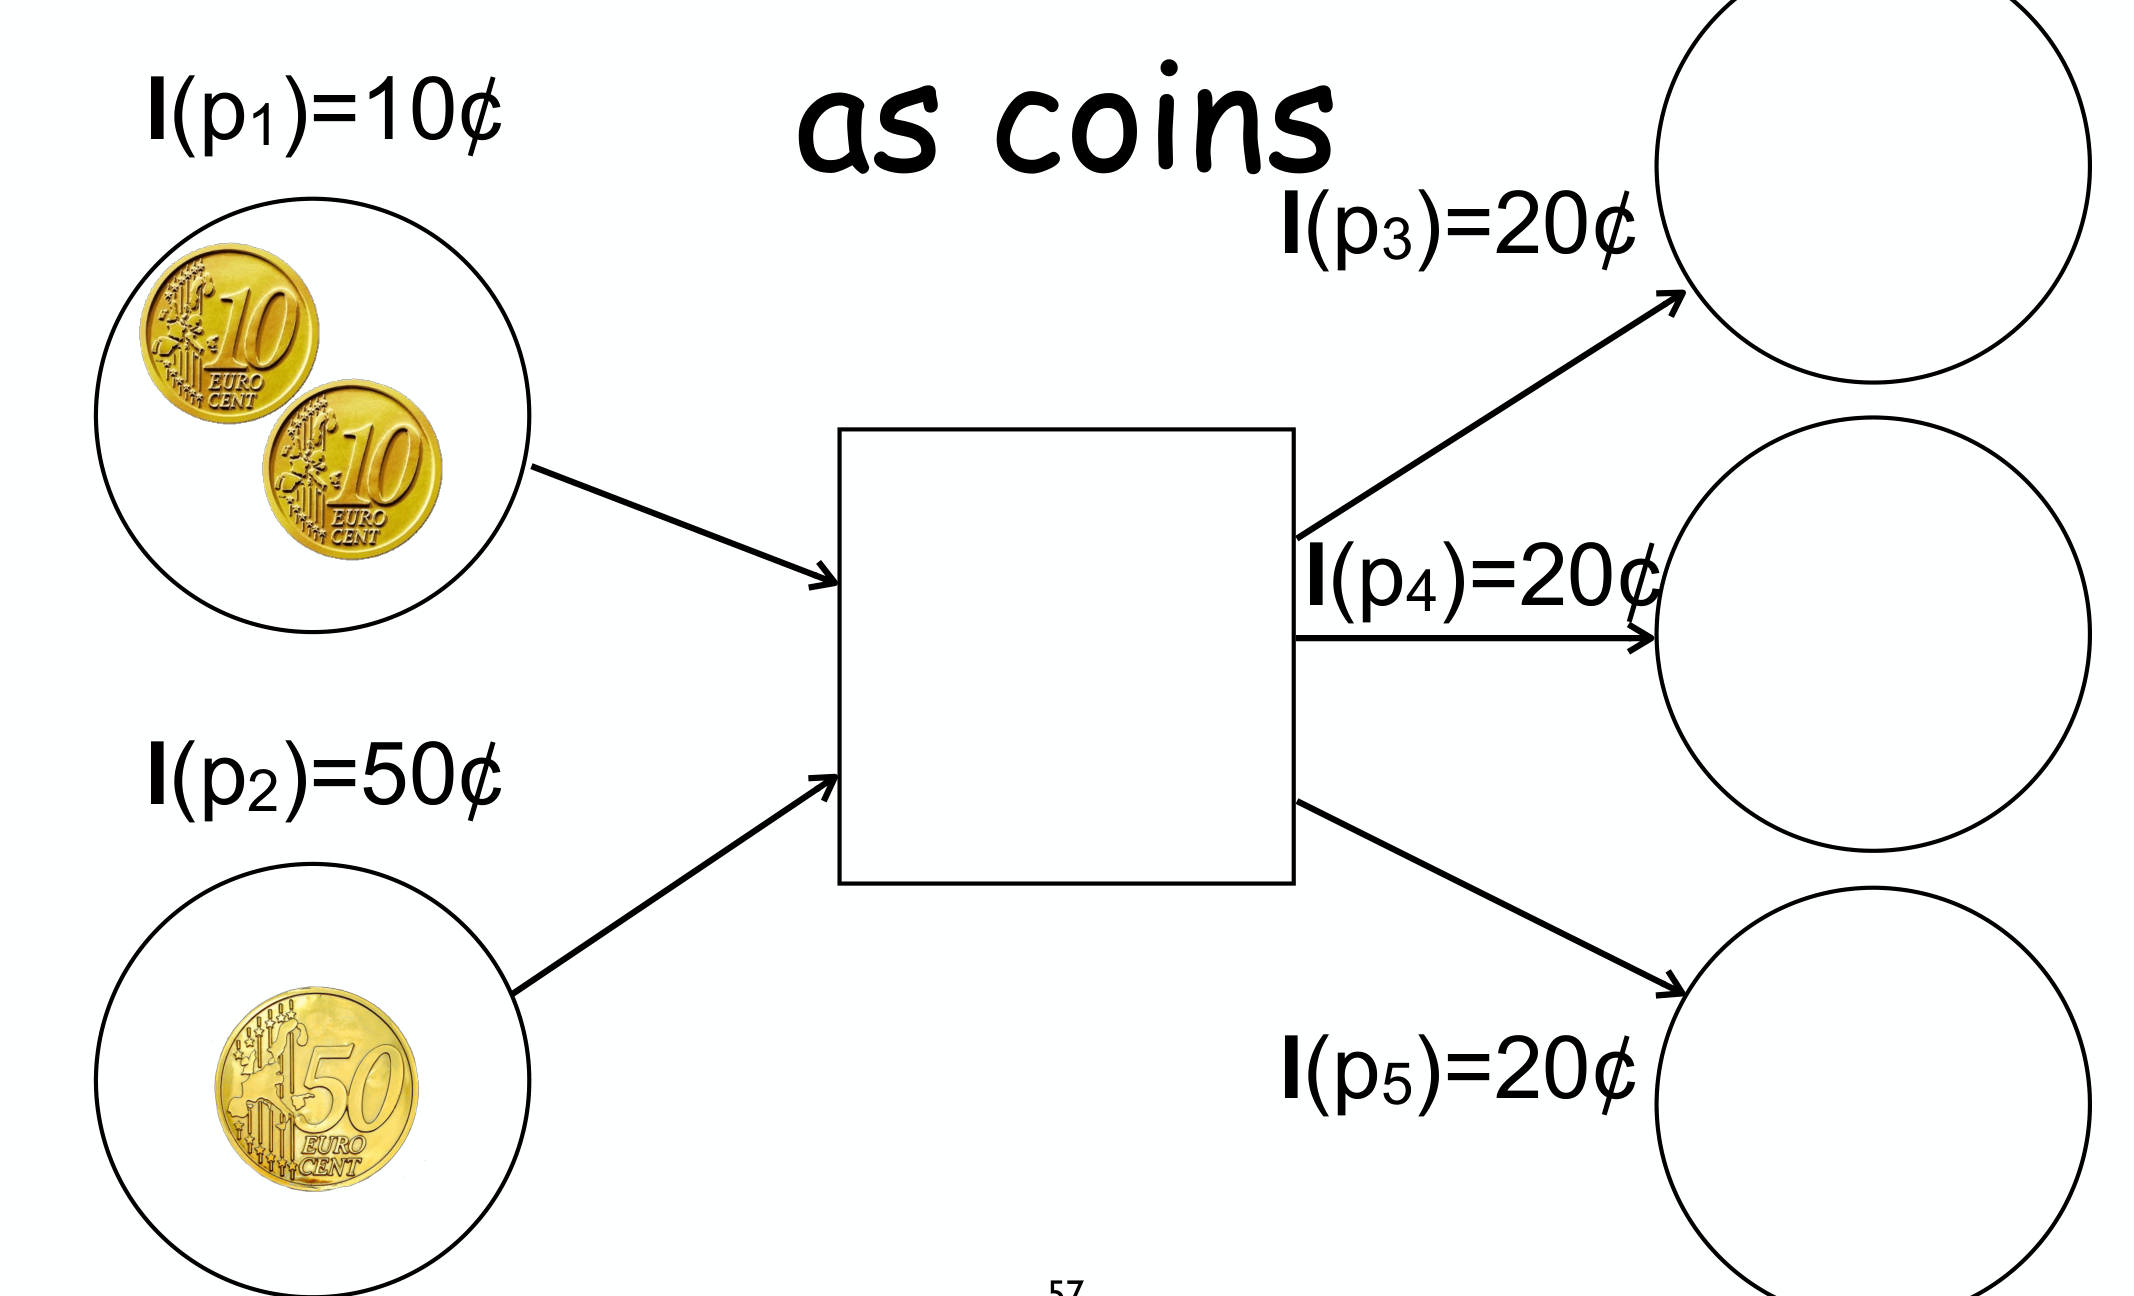
\includegraphics[width=0.74\linewidth,height=0.34\textheight,keepaspectratio]{images/14-invariants_p56_coins.png}
\caption{Token come monete. L'S-invariant $I$ assegna a ogni place un "valore". Uno scatto conserva il valore totale solo se \textbf{quello che entra vale quanto quello che esce}: qui la transizione toglie $10\text{¢}+50\text{¢} = 60\text{¢}$ e ne produce $20\text{¢} \cdot 3 = 60\text{¢}$. Se questo vale per \emph{ogni} transizione, la somma pesata dei token è un invariante.}
\end{figure}

Questa condizione "valore in ingresso = valore in uscita, per ogni transizione" si scrive in forma matriciale in modo compatto.

\begin{boxdefinition}{S-invariant}
Un \textbf{S-invariant} di una rete $N=(P,T,F)$ è un vettore $I$ (di lunghezza $|P|$, a valori razionali) che soddisfa \(I \cdot \mathbf{N} = \mathbf{0}\) dove $\mathbf{N}$ è l'incidence matrix. È un sistema lineare \textbf{omogeneo}: la soluzione banale $I = \mathbf{0}$ c'è sempre, e \textbf{ogni combinazione lineare di S-invariant è ancora un S-invariant} (quindi le soluzioni formano uno spazio vettoriale).
\end{boxdefinition}

C'è una caratterizzazione equivalente, spesso più comoda perché si legge \textbf{direttamente sul disegno} senza calcolare la matrice:

\begin{boxdefinition}{S-invariant (definizione alternativa)}
$I : P \to \mathbb{Q}$ è un S-invariant se e solo se, \textbf{per ogni transizione} $t$, il peso totale in ingresso eguaglia quello in uscita: \(\sum_{p \in \bullet t} I(p) = \sum_{p \in t\bullet} I(p)\) È esattamente la condizione "monete in = monete out" della figura, transizione per transizione.
\end{boxdefinition}

\subsection{\texorpdfstring{La proprietà fondamentale}{La proprietà fondamentale}}

Il motivo per cui gli S-invariant sono utili è un solo teorema, semplice ma potente.

\begin{boxtheorem}{Proprietà fondamentale degli S-invariant}
Se $I$ è un S-invariant, allora per \textbf{ogni} marcatura raggiungibile $M \in [M_0\rangle$: \(I \cdot M = I \cdot M_0\) Cioè la \textbf{somma pesata dei token è costante} durante tutta l'esecuzione.

\emph{Dimostrazione.} Se $M \in [M_0\rangle$, c'è $\sigma$ con $M_0 \xrightarrow{\sigma} M$. Per la marking equation (\hyperref[ch:11]{11 — Net Matrices}): \(M = M_0 + \mathbf{N}\cdot\vec{\sigma}\) Allora, moltiplicando entrambi i membri per $I$: \(I \cdot M = I \cdot M_0 + I \cdot \mathbf{N} \cdot \vec{\sigma} = I \cdot M_0 + \mathbf{0} \cdot \vec{\sigma} = I \cdot M_0\) perché $I \cdot \mathbf{N} = \mathbf{0}$. $\blacksquare$
\end{boxtheorem}

Vediamolo su un esempio concreto — il modello di due semafori — che mostra anche come \textbf{combinare} più invarianti:

\begin{figure}[!htb]
\centering
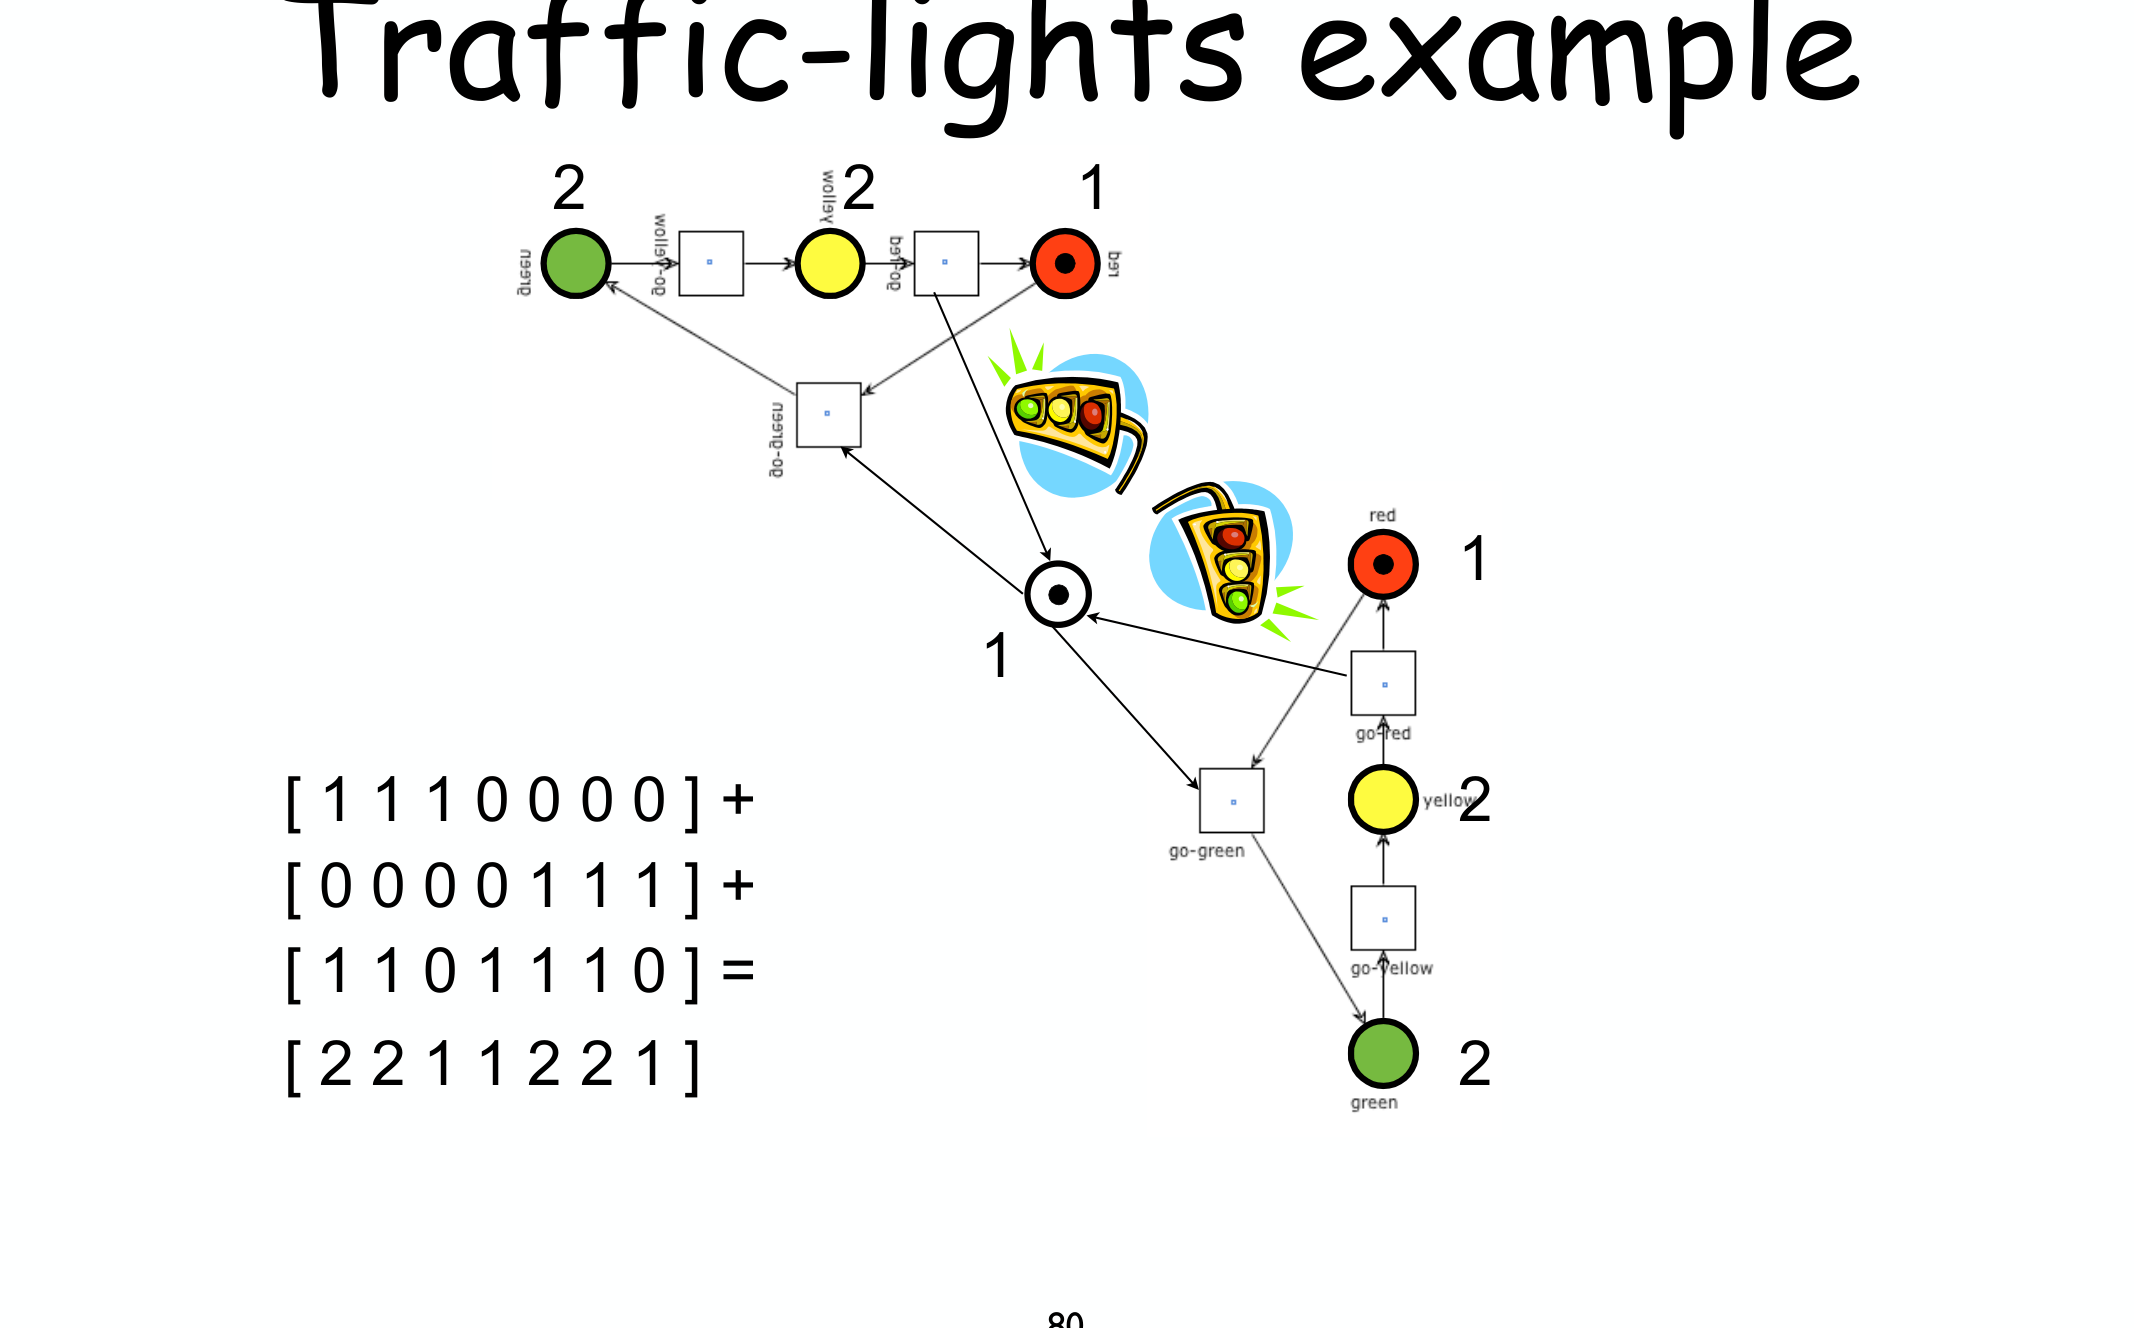
\includegraphics[width=0.74\linewidth,height=0.34\textheight,keepaspectratio]{images/14-invariants_p79_traffic-lights.png}
\caption{Esempio dei semafori. $[1\,1\,1\,0\,0\,0\,0]$ è un S-invariant: "la somma dei token nei tre place del primo semaforo è costante" (= 1, il semaforo è sempre in \emph{uno} stato). Analogamente $[0\,0\,0\,0\,1\,1\,1]$ per il secondo. Poiché le combinazioni lineari sono ancora invarianti, si possono sommare per ottenerne altri (in fondo $[2\,2\,1\,1\,2\,2\,1]$).}
\end{figure}

\subsection{\texorpdfstring{A cosa servono gli S-invariant}{A cosa servono gli S-invariant}}

Dalla proprietà fondamentale discendono tre usi pratici. Prima serve una classificazione dei possibili S-invariant, in base al segno dei pesi.

\begin{boxdefinition}{S-invariant semi-positive e positive}
\begin{itemize}
\item \textbf{Semi-positive}: $I \ge \mathbf{0}$ e $I \ne \mathbf{0}$ — nessun peso negativo, e almeno un peso strettamente positivo.
\item \textbf{Positive}: $I(p) > 0$ per \textbf{ogni} place $p$ — tutti i pesi strettamente positivi (caso più forte, implica semi-positive).
\item Il \textbf{support} $\langle I \rangle = \{p \mid I(p) > 0\}$ è l'insieme dei place con peso positivo. Per un invariante positive, il support è \textbf{tutto} $P$.
\end{itemize}
\end{boxdefinition}

\begin{boxtheorem}{1) Boundedness (condizione sufficiente)}
Se la rete ha un S-invariant \textbf{positive}, allora è \textbf{bounded}. Anzi, ogni place è limitato esplicitamente: da \(I(p)\,M(p) \le I\cdot M = I\cdot M_0\) segue \(M(p) \le \frac{I \cdot M_0}{I(p)}\) un limite \textbf{indipendente} dalla marcatura raggiungibile. Basta dunque \emph{esibire} un S-invariant positive per certificare la boundedness — senza esplorare gli stati.
\end{boxtheorem}

\begin{boxtheorem}{2) Disprovare la liveness}
Se la rete è \textbf{live}, allora per ogni S-invariant semi-positive $I$ vale $I \cdot M_0 > 0$. Per contrapposizione: \textbf{se troviamo un S-invariant semi-positive con $I \cdot M_0 = 0$, la rete non è live.} (Se il valore iniziale è zero e i pesi sono $\ge 0$, i place del support restano vuoti per sempre $\rightarrow$ le transizioni collegate sono dead.)
\end{boxtheorem}

\begin{boxtheorem}{3) Disprovare la raggiungibilità}
Poiché $I \cdot M = I \cdot M_0$ per ogni $M$ raggiungibile, \textbf{se una marcatura $M$ ha $I \cdot M \ne I \cdot M_0$ per qualche S-invariant $I$, allora $M$ non è raggiungibile.} È un test veloce che evita di risolvere il problema di raggiungibilità completo (EXPSPACE-hard).
\end{boxtheorem}

\begin{boxwarning}{Le implicazioni non si invertono}
Attenzione: sono condizioni \emph{sufficienti} o \emph{necessarie}, non equivalenze. \textbf{Niente} S-invariant positive $\Longrightarrow$ \emph{forse} unbounded (non è detto). $I \cdot M_0 > 0$ $\Longrightarrow$ \emph{forse} live. $I \cdot M = I \cdot M_0$ $\Longrightarrow$ \emph{forse} $M$ raggiungibile. Gli invarianti danno certezze solo "in un verso".
\end{boxwarning}

\section{\texorpdfstring{T-invariant: il ragionamento duale}{T-invariant: il ragionamento duale}}

Gli S-invariant nascono dall'equazione $I \cdot \mathbf{N} = \mathbf{0}$ (vettori a sinistra della matrice). Viene naturale chiedersi cosa si ottiene dall'equazione \textbf{duale}, con i vettori a destra: $\mathbf{N} \cdot y = \mathbf{0}$.

\begin{boxdefinition}{T-invariant}
Un \textbf{T-invariant} (o \emph{transition-invariant}) di $N=(P,T,F)$ è un vettore $J$ (di lunghezza $|T|$, razionale) che soddisfa \(\mathbf{N} \cdot J = \mathbf{0}\) La caratterizzazione alternativa, leggibile sul disegno: $J$ è un T-invariant se e solo se \textbf{per ogni place} $p$, $\sum_{t \in \bullet p} J(t) = \sum_{t \in p\bullet} J(t)$ (i token prodotti in $p$ eguagliano quelli consumati).
\end{boxdefinition}

Mentre un S-invariant è un peso \emph{sui place} con significato "valore conservato", un T-invariant è un conteggio \emph{sulle transizioni} con un significato diverso e altrettanto elegante.

\begin{boxtheorem}{Proprietà fondamentale dei T-invariant}
Sia $M \xrightarrow{\sigma} M'$. Il Parikh vector $\vec{\sigma}$ è un T-invariant \textbf{se e solo se} $M' = M$.

In parole: un T-invariant è \textbf{un insieme di scatti (con molteplicità) che riporta la rete esattamente alla marcatura di partenza}. La dimostrazione è immediata dalla marking equation: \(M' = M + \mathbf{N}\cdot\vec{\sigma}\) quindi \(M' = M \iff \mathbf{N}\cdot\vec{\sigma} = \mathbf{0}\)
\end{boxtheorem}

\begin{figure}[!htb]
\centering
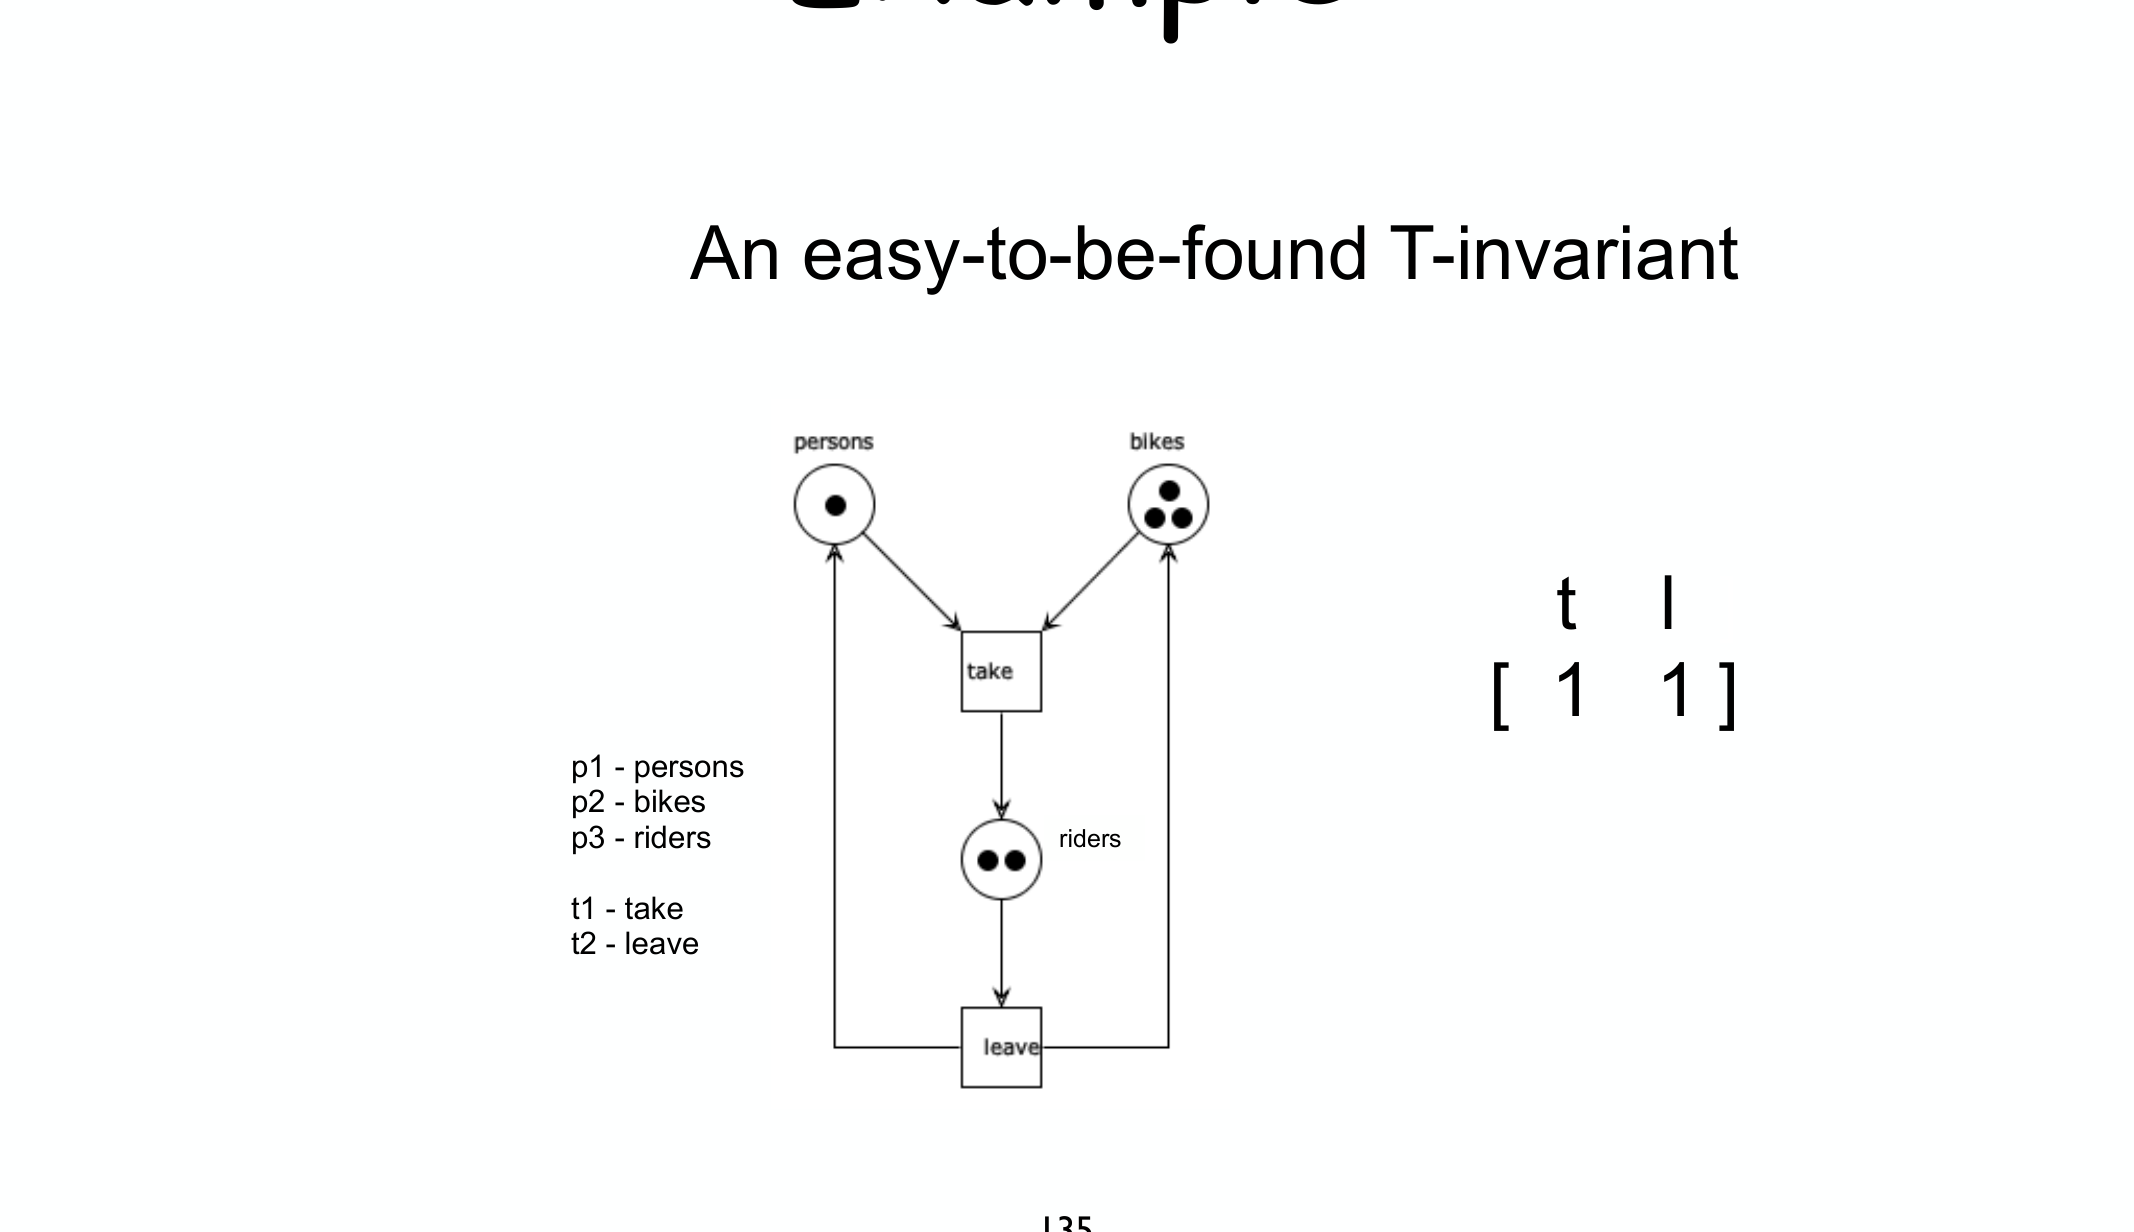
\includegraphics[width=0.74\linewidth,height=0.34\textheight,keepaspectratio]{images/14-invariants_p134_t-invariant.png}
\caption{Un T-invariant facile da trovare. Nella rete "noleggio bici", \texttt{take} (persona+bici $\rightarrow$ rider) e \texttt{leave} (rider $\rightarrow$ persona+bici) sono l'una l'inversa dell'altra: il T-invariant $J = [1,1]$ dice che \textbf{eseguendo \texttt{take} una volta e \texttt{leave} una volta si torna allo stato di partenza}. L'ordine non conta (il Parikh vector lo dimentica).}
\end{figure}

\subsection{\texorpdfstring{A cosa servono i T-invariant}{A cosa servono i T-invariant}}

Il risultato chiave lega T-invariant, boundedness e liveness, e usa il \textbf{principio dei cassetti} (pigeonhole): se un cammino attraversa più stati di quanti ne esistano, uno stato si ripete.

\begin{boxtheorem}{Bounded + live $\Longrightarrow$ positive T-invariant}
Se un sistema \textbf{bounded} ha una sequenza infinita di scatti (cosa garantita dalla liveness), allora — poiché gli stati raggiungibili sono finiti — per il pigeonhole una marcatura $M_i$ si ripete: \(M_i \xrightarrow{\sigma'} M_j = M_i\) Il Parikh vector di $\sigma'$ è un T-invariant (\emph{reproduction lemma}). Con la liveness si può fare in modo che coinvolga \emph{tutte} le transizioni, ottenendo un T-invariant \textbf{positive}.
\end{boxtheorem}

Per contrapposizione si ricavano test utili:

\begin{boxnote}{Usi dei T-invariant}
\begin{itemize}
\item \textbf{Disprovare la boundedness}: un sistema \emph{live} \textbf{senza} T-invariant positive è \textbf{unbounded}.
\item \textbf{Disprovare la liveness}: un sistema \emph{bounded} \textbf{senza} T-invariant positive è \textbf{non-live}. (In particolare, se una rete ha un S-invariant positive — quindi è bounded — ma nessun T-invariant positive, allora \textbf{non può essere live}.)
\item In generale, \textbf{nessun T-invariant positive $\Longrightarrow$ non (live e bounded)}: o è non-live, o è unbounded.
\end{itemize}
\end{boxnote}

\section{\texorpdfstring{Il quadro d'insieme: S- e T-invariant insieme}{Il quadro d'insieme: S- e T-invariant insieme}}

I due tipi di invariante sono complementari e, presi insieme, dicono molto sulla struttura globale della rete.

\begin{boxtheorem}{Strong connectedness via invarianti}
Se una rete \textbf{weakly connected} ha \textbf{sia} un S-invariant positive \textbf{sia} un T-invariant positive, allora è \textbf{strongly connected}.

Conseguenza (contrapposta): una rete weakly connected ma \textbf{non} strongly connected non può avere entrambi. Combinato con quanto visto in \hyperref[ch:12]{12 — Soundness} (weakly connected + live + bounded $\Longrightarrow$ strongly connected), questo dà criteri strutturali rapidi per escludere soundness e altre buone proprietà.
\end{boxtheorem}

\begin{boxabstract}{Riepilogo: cosa provano gli invarianti}
\begingroup\small
\begin{tabularx}{\linewidth}{>{\raggedright\arraybackslash}X>{\raggedright\arraybackslash}X>{\raggedright\arraybackslash}X}
\toprule
\textbf{Strumento} & \textbf{Prova / dimostra} & \textbf{Come} \\
\midrule
\textbf{S-invariant positive} & boundedness & esibirne uno \\
\textbf{S-invariant semi-positive} con $I\cdot M_0 = 0$ & non-liveness & esibirne uno \\
\textbf{S-invariant} con $I\cdot M \ne I\cdot M_0$ & $M$ non raggiungibile & esibirne uno \\
\textbf{T-invariant positive} (assente, con liveness) & unboundedness & mostrarne l'assenza \\
\textbf{T-invariant positive} (assente, con boundedness) & non-liveness & mostrarne l'assenza \\
\bottomrule
\end{tabularx}
\endgroup

Il filo conduttore: gli invarianti trasformano domande sul \emph{comportamento} (esplorare infiniti stati) in \textbf{calcoli di algebra lineare} sulla struttura.
\end{boxabstract}

Gli invarianti sono l'apice degli strumenti algebrici del corso. Le prossime lezioni li applicano a classi speciali di reti (come i sistemi S e T) e all'analisi dei processi. $\rightarrow$ \hyperref[ch:15]{15 — S-T Systems}